\documentclass[UTF8]{ctexart}
\usepackage{amsmath}
\usepackage{amssymb}
\usepackage{background}
\usepackage{booktabs}
\usepackage{caption,subcaption}
\usepackage{enumitem}
\usepackage{float}
\usepackage{fontspec}
\usepackage{geometry}
\usepackage{makecell}
\usepackage{mathptmx} %mathptmx和times结合使得公式使用times new roman字体
\usepackage{tcolorbox}
\tcbuselibrary{breakable, raster}
\usepackage{tikz}
\usetikzlibrary{arrows.meta}
\usepackage{times}
\usepackage{xcolor}

\geometry{a5paper, top=0.1cm, left=1cm, right=1cm, bottom=1cm, footskip=0.6cm, marginparsep=0.1cm}

\setCJKmainfont[BoldFont={汉仪文黑-85W},ItalicFont={方正苏新诗柳楷简体}]{汉仪文黑-55W}
\setfontfamily\Issue{Century Schoolbook}
\setfontfamily\Genshin{Genshin Teyvat Lingua Franca}
\newfontfamily\timesnewroman{Times New Roman}
\setmainfont{Times New Roman}
\newCJKfontfamily\TitleFont{思源宋体 CN Heavy}
\captionsetup{font=small, labelfont=bf}
\setlist[itemize]{itemsep=0pt, parsep=0pt}
%\reversemarginpar

%\CTEXsetup[format = {\centering\bfseries\large}, beforeskip = 3pt, afterskip = 3pt]{section}
\CTEXsetup[format = {\color{cyan!50!black}\bfseries\large}]{subsection}

\newtcolorbox{mybox}{colback=cyan!10, colframe=cyan!50!black, boxrule=0.5pt, breakable}

\colorlet{darkcyan}{cyan!50!black}
\newcommand\Black[1]{\textcolor[gray]{0.3}{#1}}
\newcommand\Brown[1]{\textcolor[HTML]{998A4E}{#1}}
\newcommand\Emph[1]{\colorbox{green!10}{\textcolor{green!30!black}{#1}}}
\newcommand\Concept[1]{\textcolor{cyan!70!black}{#1}}
\newcommand\Notes[1]{\textcolor{yellow!50!black}{\small #1}}
\newcommand\Example[1]{\textcolor{cyan!70!black}{\small #1}}
\newcommand\means[1]{\textcolor{cyan!70!black}{#1}}

\newcommand\Ohm{\text{\timesnewroman Ω}}

\newcommand\IssueNumber{26}
\newcommand\Date{2024-5-11}
%\newcommand\Contributer{@金光日}
\newcommand\Subject{数字逻辑}
%\newcommand\Source{2022 考研 408 第 5 题}


\begin{document}
\backgroundsetup{contents=
\includegraphics{上半示例.png}, center, scale=1, angle=0, opacity=1}
\BgThispage
\begin{center}
%{\scriptsize\Issue \textcolor[HTML]{C8BA83}{\Genshin WEEKLY TIPS}}
\phantom{...}

{\Large\textcolor{brown!40!white}{\makebox[10cm][s]{\Genshin WEEKLY KNOWLEDGE TIPS}}}

\vspace{-2em}

{\Huge\bfseries\TitleFont \Black{知\ 识\ 小\ 料}}


\vspace{-0.1cm}
{\footnotesize \Brown{「电计 2203 班」周常规知识整理共享}}
\end{center}

\vspace{-0.5cm}


\begin{figure}[H]
\hspace{1cm}
\begin{minipage}[t]{0.3\textwidth}
\centering
    \Brown{\Genshin ISSUE}

    \vspace{-0.6cm}
    \Huge \Issue\slshape\bfseries\Black{\IssueNumber}
\end{minipage}
\hfill
\begin{minipage}[t]{0.35\textwidth}
\small
\centering
    \Brown{日期:\Date} \\
%\vspace{-0.1cm}
%    \Brown{贡献者:\Contributer} \\
\vspace{-0.1cm}
    \Brown{学科:\Subject} \\
%\vspace{-0.1cm}
%    \Brown{来源:\Source}
\end{minipage}
\hspace{0.8cm}
\end{figure}

{\color{cyan!50!black}
如题所示,是两个 555 定时器构成的电路。在开关 K 按下以后,扬声器 TH 以频率 200Hz 响 2s。
\begin{enumerate}[itemsep=0pt,parsep=0pt]
  \item 请指出 555(I)和 555(II)功能;
  \item 请计算电阻 $R_1$ 的值;
  \item 请计算电阻 $R_2$ 的值。
\end{enumerate}
\begin{figure}[htb]
  \centering
  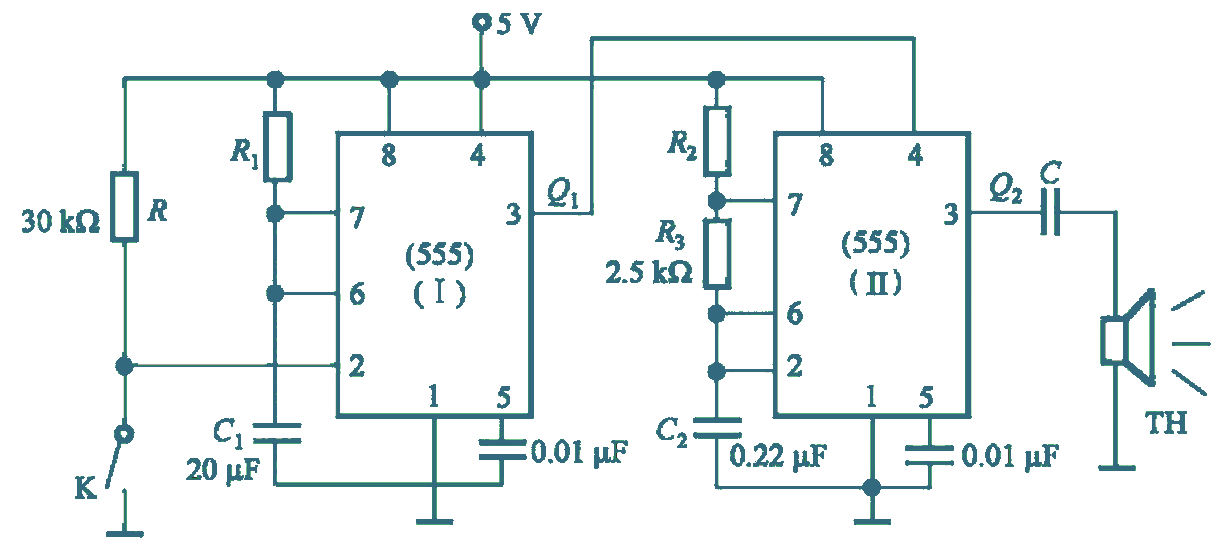
\includegraphics[width=10cm]{题目-1.png}
\end{figure}
}

【第 1 题】观察两个芯片,555(I) 的 6,7 脚接在一起,2 脚作输入,因此是\textcolor{blue}{单稳态触发器};555(II) 的 2,6 脚接在一起,因此是\textcolor{blue}{多谐振荡器}。

\begin{itemize}[itemsep=0pt,parsep=0pt]
  \item 当芯片 (I) 输出 $Q_1=1$,(II) 也随之工作,电路会响 2s;
  \item 当芯片 (I) 输出 $Q_1=0$,(II) 的 4 脚接低电平,故复位不工作。
\end{itemize}


【第 2 题】芯片 (I) 控制整个电路是否在振荡,因此用到的是 2s 的条件。利用单稳态触发器的振荡周期式
\begin{equation}\label{eq:1}
  \color{blue} T_1 = 1.1R_1C_1 = 2\mathrm{s}
\end{equation}
\begin{equation*}
  R_1 = \frac{2}{1.1\times 20\times 10^{-6}} = 91\mathrm{k\Ohm}
\end{equation*}

\newpage
\backgroundsetup{contents=
\includegraphics{下半示例.png}, center, scale=1, angle=0, opacity=1}
\BgThispage

【第 3 题】芯片 (II) 控制振荡的频率和周期,因此用到的是 200Hz 的条件。由多谐振荡器的周期,充电周期 $T_\text{充} = 0.7(R_2+R_3)C_2$,放电周期 $T_\text{放} = 0.7R_3C_2$,得到总周期
\begin{equation}\label{eq:2}
  \color{blue} T_2 = 0.7(R_2+2R_3)C_2 = \frac{1}{200\mathrm{Hz}} = 5\times 10^{-3}\mathrm{s}
\end{equation}
\begin{equation*}
  R_2 = \frac{5\times 10^{-3}}{0.7\times 0.22\times 10^{-6}} - (2\times 2.5\times 10^3) = 27.5\mathrm{k\Omega}
\end{equation*}

补充一下,这道题的波形大致是这样的\textcolor{cyan}{(仅为示意图,不反映真实比例)}:
\begin{figure}[htb]
  \centering
  \begin{tikzpicture}[>=Stealth]
    \draw[color=lightgray, ->] (-0.5,-0.1) -- (8.5,-0.1) node[above] {$t$};
    \draw[color=lightgray, ->] (-0.5,-0.1) -- (-0.5,1.5) node[left] {$Q_2$};
    \node[color=lightgray, left] at (-0.5,-0.1) {$O$}; 
    \draw (-0.5,0) -- (0,0);
    \foreach \x in {0,0.1,...,2}{
        \draw (\x,0) -- (\x+0.05,0) -- (\x+0.05, 1) -- (\x+0.1, 1) -- (\x+0.1, 0);
    }
    \draw (2, 0) -- (5,0);
    \draw[->] (0.05, -1) node[below,font=\footnotesize]{按开关} -- (0.05 ,0);
    \draw[<->, color=cyan!80!black] (0.05, -0.5) -- node[midway,above]{2s} (2, -0.5);
    \draw[color=cyan!80!black] (2,-0.3) -- (2,-0.6);
    \foreach \x in {5,5.1,...,7}{
        \draw (\x,0) -- (\x+0.05,0) -- (\x+0.05, 1) -- (\x+0.1, 1) -- (\x+0.1, 0);
    }
    \draw (7, 0) -- (8,0);
    \draw[->] (5.05, -1) node[below,font=\footnotesize]{按开关} -- (5.05 ,0);
    \draw[color=cyan!80!black] (5.05, 1.2) --node[midway, above, outer sep=3pt]{$5\times 10^{-3}\mathrm{s}$(200Hz)} (5.15, 1.2);
    \draw[color=cyan!80!black, ->] (4.5, 1.2) -- (5.05, 1.2);
    \draw[color=cyan!80!black, ->] (5.7, 1.2) -- (5.15, 1.2);
    \draw[color=cyan!80!black] (5.05, 1.1) -- (5.05, 1.4);
    \draw[color=cyan!80!black] (5.15, 1.1) -- (5.15, 1.4);
  \end{tikzpicture}
\end{figure}

{\color{cyan!80!black} 【结论】1. 555(I) 作单稳态触发器,555(II) 作多谐振荡器;2. $R_1 = \mathrm{91k\Ohm}$;3. $R_2 = 27.5\mathrm{k\Ohm}$。

【点评】本题考察了第七章《脉冲波形的产生与变换》的单稳态触发器、多谐振荡器的内容,需要同学们能够识别 555 定时器的功能,以及其典型应用——施密特触发器、单稳态触发器、多谐振荡器等。
}


\end{document} 